\documentclass[a4paper,14pt]{report} % формат документа

\usepackage{cmap} % поиск в ПДФ
\usepackage[T2A]{fontenc} % кодировка
\usepackage[utf8]{inputenc} % кодировка исходного текста
\usepackage[english,russian]{babel} % локализация и переносы
\usepackage[left = 2cm, right = 1cm, top = 2cm, bottom = 2 cm]{geometry} % поля
\usepackage{listings}
\usepackage{graphicx} % для вставки рисунков
\graphicspath{{pictures/}}
\DeclareGraphicsExtensions{.pdf,.png,.jpg}

\lstset{ %
  language=Python,                % Язык программирования 
  numbers=left,                   % С какой стороны нумеровать          
  frame=single,                    % Добавить рамку
}

\author{Сиденко Анастасия}
\title{Лабораторная работа 1}
\date{\today}

\begin{document}
\maketitle
\tableofcontents
\renewcommand{\chaptername}{Часть}

\chapter{Введение}
\section{Постановка задачи}
Алгоритмы поиска расстояний:
\begin{enumerate} 
  \item Левенштейна
  \item  Дамерау-Левенштейна
\end{enumerate} 
Способы реализации:
\begin{enumerate} 
  \item матричный
  \item  рекурсивный
\end{enumerate} 

\chapter{Аналитическая часть}
\section{Расстояние Левенштейна и Дамерау-Левенштейна}

\textbf{Расстояние Левенштейна} или редакционное расстояние между строками двумя стрками - это минимальное количество редакторских операций, необходимых для преобразования первой строки во вторую. 

\textbf{Редакторские операции: }
\begin{enumerate}
  \item I -- Вставка -- штраф 1
  \item D -- Удаление -- штраф 1
  \item R -- Замена -- штраф 1
  \item M -- Совпадение -- штраф 0
\end{enumerate}

\textbf{Расстояние Дамерау-Левенштейна} - расширение, вводится операция транспозиции или перестановки 2 соседних символов (штраф 1). 

\chapter{Конструкторская часть}
\section{Алгоритмы}

$$D(S_1[1...i], S_2[1...j]) = 
\left\{
  \begin{array}{lll}
    D(S_1[1...i], S_2[1...j - 1] + 1) - Insert \\
    D(S_1[1...i - 1], S_2[1...j] + 1) - Delete \\
    D(S_1[1...i - 1], S_2[1...j - 1] + 
    \left[
        \begin{array}{lll}
         0,~ if ~S_1[i] = S_2[j] - Match\\
         1, ~else - Replace \\
         \end{array}
    \right.
  \end{array}
\right.$$

Если используется модифицированное расстояние, то добавляется дополнительное условие:\\
$$D(S_1[1...i - 2], S_2[1...j - 2] + 1, ~ if ~S_1[i] = S_2[j - 1] ~and ~S_1[i - 1] = S_2[j ]$$

\textbf{Способы: }
\begin{enumerate}
  \item Матричный:\\
  При матричном способе для каждой следующей клетки выбирается минимальное расстояние в одном из укзанных направлений:
  \begin{figure}[h]
  \center{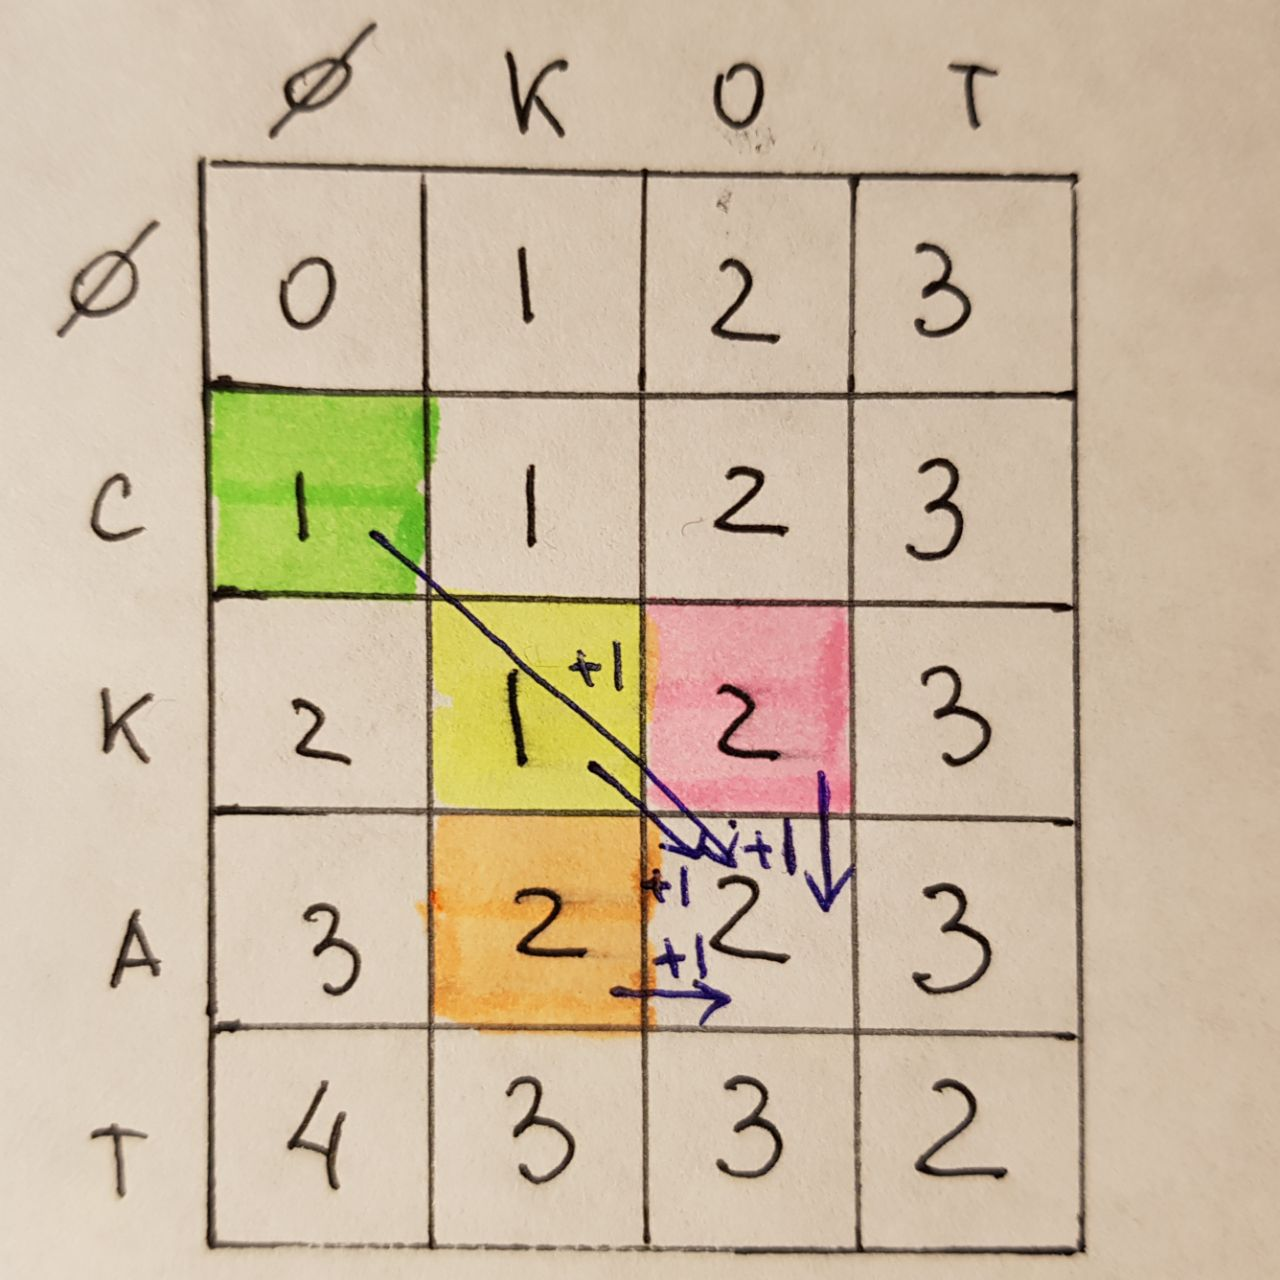
\includegraphics[scale=0.1]{matrix}}
  \end{figure} 
  \item Рекурсивный:\\
  Раскрываем рекурсивно по формулам каждую из 4 операций. 
\end{enumerate}

\chapter{Технологическая часть}
\section{Листинг кода}

\textbf{Расстояние Левинштейна, матричный способ: }
\begin{lstlisting}
def levinstein(s1, s2):
    n_matrix = len(s1) + 1
    m_matrix = len(s2) + 1
    matrix = [[0] * m_matrix for i in range(n_matrix)]

    for i in range(n_matrix):
        matrix[i][0] = i
    for j in range(m_matrix):
        matrix[0][j] = j

    for i in range(1, n_matrix):
        for j in range(1, m_matrix):
            matrix[i][j] = min(matrix[i - 1][j] + 1, matrix[i][j - 1] + 1,
            matrix[i - 1][j - 1] + (s1[i - 1] != s2[j - 1]))

    for i in range(n_matrix):
        for j in range(m_matrix):
            print(matrix[i][j], end = ' ')
        print()
    return matrix[n_matrix - 1][m_matrix - 1]
\end{lstlisting}

\textbf{Расстояние Дамерау-Левинштейна, матричный способ: }
\begin{lstlisting}
def damerau_levinstein_matrix(s1, s2):
    n_matrix = len(s1) + 1
    m_matrix = len(s2) + 1
    matrix = [[0] * m_matrix for i in range(n_matrix)]

    for i in range(n_matrix):
        matrix[i][0] = i
    for j in range(m_matrix):
        matrix[0][j] = j

    for i in range(1, n_matrix):
        for j in range(1, m_matrix):
            if (i > 1 and s1[i - 1] == s2[j - 2] and s1[i - 2] == s2[j - 1]):
                matrix[i][j] = min(matrix[i - 1][j] + 1, matrix[i][j - 1] + 1,
                matrix[i - 1][j - 1] + (s1[i - 1] != s2[j - 1]), matrix[i - 2][j - 2] + 1)
            else:
                matrix[i][j] = min(matrix[i - 1][j] + 1, matrix[i][j - 1] + 1,
                matrix[i - 1][j - 1] + (s1[i - 1] != s2[j - 1]))

    for i in range(n_matrix):
        for j in range(m_matrix):
            print(matrix[i][j], end = ' ')
        print()
    return matrix[n_matrix - 1][m_matrix - 1]
\end{lstlisting}

\textbf{Расстояние Дамерау-Левинштейна, рекурсивный способ: }
\begin{lstlisting}
def damerau_levinstein_recursive(s1, s2):
    n = len(s1)
    m = len(s2)
    if (0 == n):
        return m
    if (0 == m):
        return n

    delete = damerau_levinstein_recursive(s1[:-1], s2) + 1
    insert = damerau_levinstein_recursive(s1, s2[:-1]) + 1
    replace = damerau_levinstein_recursive(s1[:-1], s2[:-1]) + (s1[-1] != s2[-1])
    transposition = 1000
    if (n > 1 and m > 1 and s1[-1] == s2[-2] and s1[-2] == s2[-1]):
        transposition = damerau_levinstein_recursive(s1[:-2], s2[:-2]) + 1

    return min(delete, insert, replace, transposition)
\end{lstlisting}

\section{Заготовленные тесты}

\begin{tabular}{ | l | l | l |}
\hline
\textbf{Строка1} & \textbf{Строка2} & \textbf{Ожидаемый результат} \\ \hline
dessert & desert & 1 \\ \hline
cook & cooker & 2 \\ \hline
mother & money & 3 \\ \hline
woman & water & 4 \\ \hline
program & friend & 6 \\ \hline
house & girl & 5 \\ \hline
probelm & problem & 1 or 2 \\ \hline
head & ehda & 2 or 3 \\ \hline
bring & brought & 4 \\ \hline
happy & happy & 0\\  \hline
minute & moment & 5 \\ \hline
person & eye & 5 \\ \hline
week & weeks & 1 \\ \hline
member & morning & 6 \\ \hline
death & health & 2 \\ \hline
education & question & 4 \\ \hline
room & moor & 2 \\ \hline
car & city & 3 \\ \hline
air & area & 3 \\ \hline
country & office & 6 \\ \hline
\end{tabular}

\chapter{Экспериментальная(исследовательская) часть}
\section{Результаты тестов}

\begin{tabular}{ | l | l | l | l | l |}
\hline
\textbf{Строка1} & \textbf{Строка2} & \textbf{Л. матричный} & \textbf{Д.-Л. матричный}  & \textbf{Д.-Л. рекурсивный}\\ \hline
dessert  &  desert  &  1  &  1  &  1 \\ \hline
cook  &  cooker  &  2  &  2  &  2 \\ \hline
mother  &  money  &  3  &  3  &  3 \\ \hline
woman  &  water  &  4  &  4  &  4 \\ \hline
program  &  friend  &  6  &  6  &  6 \\ \hline
house  &  girl  &  5  &  5  &  5 \\ \hline
probelm  &  problem  &  2  &  1  &  1 \\ \hline
head  &  ehda  &  3  &  2  &  2 \\ \hline
bring  &  brought  &  4  &  4  &  4 \\ \hline
happy  &  happy  &  0  &  0  &  0 \\ \hline
minute  &  moment  &  5  &  5  &  5 \\ \hline
person  &  eye  &  5  &  5  &  5 \\ \hline
week  &  weeks  &  1  &  1  &  1 \\ \hline
member  &  morning  &  6  &  6  &  6 \\ \hline
death  &  health  &  2  &  2  &  2 \\ \hline
education  &  question  &  4  &  4  &  4 \\ \hline
room  &  moor  &  2  &  2  &  2 \\ \hline
car  &  city  &  3  &  3  &  3 \\ \hline
air  &  area  &  3  &  3  &  3 \\ \hline
country  &  office  &  6  &  6  &  6 \\ \hline
\end{tabular}

\textbf{Тесты пройдены}

\section{Замеры времени (графики зависимости времени от длины слова)}

\textbf{Графики:}
\begin{enumerate}
  \item Левенштейн матричный -- \textbf{красный} \\
  \item Дамерау-Левенштейн матричный -- \textbf{желтый}\\
  \item Дамерау-Левенштейн рекурсивный -- \textbf{синий}
\end{enumerate}

  \begin{figure}[h]
  \center{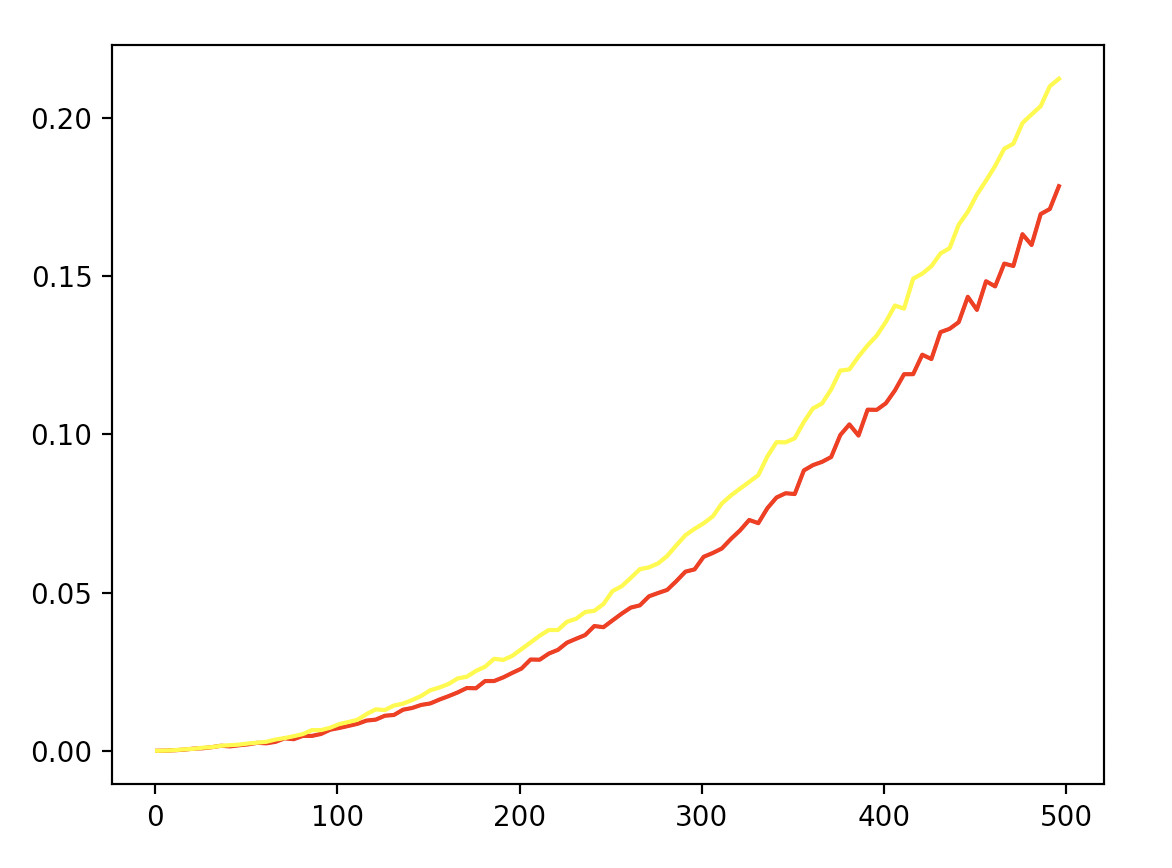
\includegraphics[scale=0.8]{plot1} \\ Левенштейн и Дамерау-Левенштейн матричный}
  \end{figure} 
  
    \begin{figure}[h]
  \center{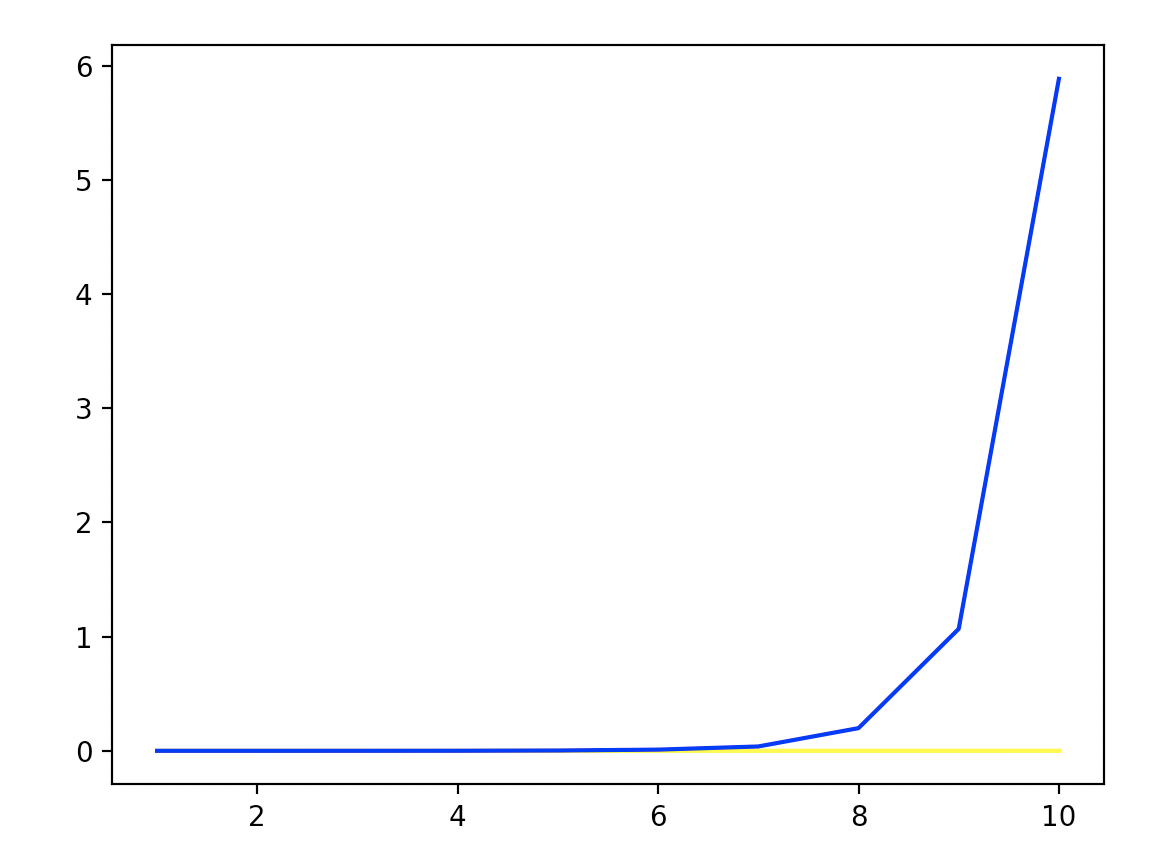
\includegraphics[scale=0.8]{plot2} \\ Дамерау-Левенштейн матричный и рекурсивный}
  \end{figure} 
  
    \begin{figure}[h]
  \center{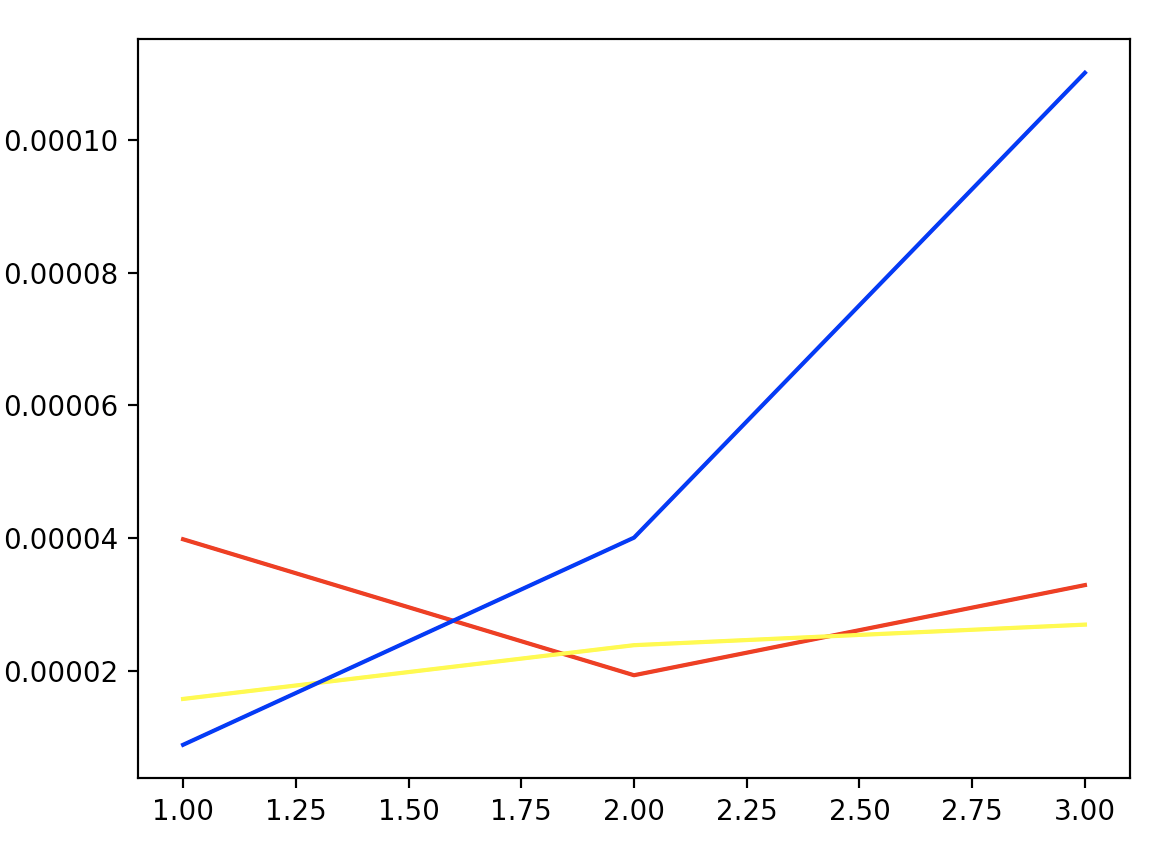
\includegraphics[scale=0.8]{plot3} \\ Все 3 способа}
  \end{figure} 

\chapter{Заключение}

В данной лабораторной работе было реализовано 3 алгоритма:
\begin{enumerate}
  \item нахождение расстояния Левенштейна матричным способом \\
  \item нахождение расстояния Дамерау-Левенштейна матричным способом \\
  \item нахождение расстояния Дамерау-Левенштейна рекурсивным способом \\
\end{enumerate}
Применяются данные алгоритмы:
\begin{enumerate}
  \item компьютерная, машинная лингвистика \\
  \item биоинформатика \\
\end{enumerate}

При сравнении данных алгоритмов были получены следующие результаты:
\begin{enumerate}
  \item Рекурсивный алгоритм является самым медленным, гораздо быстрее использовать алгоритмы матричные.   \\
  \item Дамерау-Левенштейна проигрывает обычному Левенштейну только на очень больших длинах слов, но цена ошибки, в некоторых случаях, у него меньше.\\
\end{enumerate}
\end{document}
